DARWIN is a high-level description of an algorithm, that can be used to solve
a~multi-objective optimization problem. It is a~list steps to execute and
calculations to perform. Therefore, one does not need a computer to realize
the decision-making process. However, in practise it is almost impossible to
complete all the steps without a dedicated software application. Moreover, to
evaluate the method's performance one needs to repeat the experiments many
times over and over again.

For the reasons stated above it was required to implement the method on a
computer system. This chapter describes technologies used for the DARWIN's
implementation and an experiment framework development.

\section{The method's implementation}

\subsection{The environment}

The environment, in which DARWIN has to function is not empty; thus has to be
taken into account during the development of the implementation. It is shown
in~fig.~\ref{environ}. Darwin is a~realisation of an interactive process,
therefore a way of complication with the decision maker is required. Another
restriction is imposed by the need of inducing decision rules from the sorted
examples of solutions.

\begin{figure}
  \centering 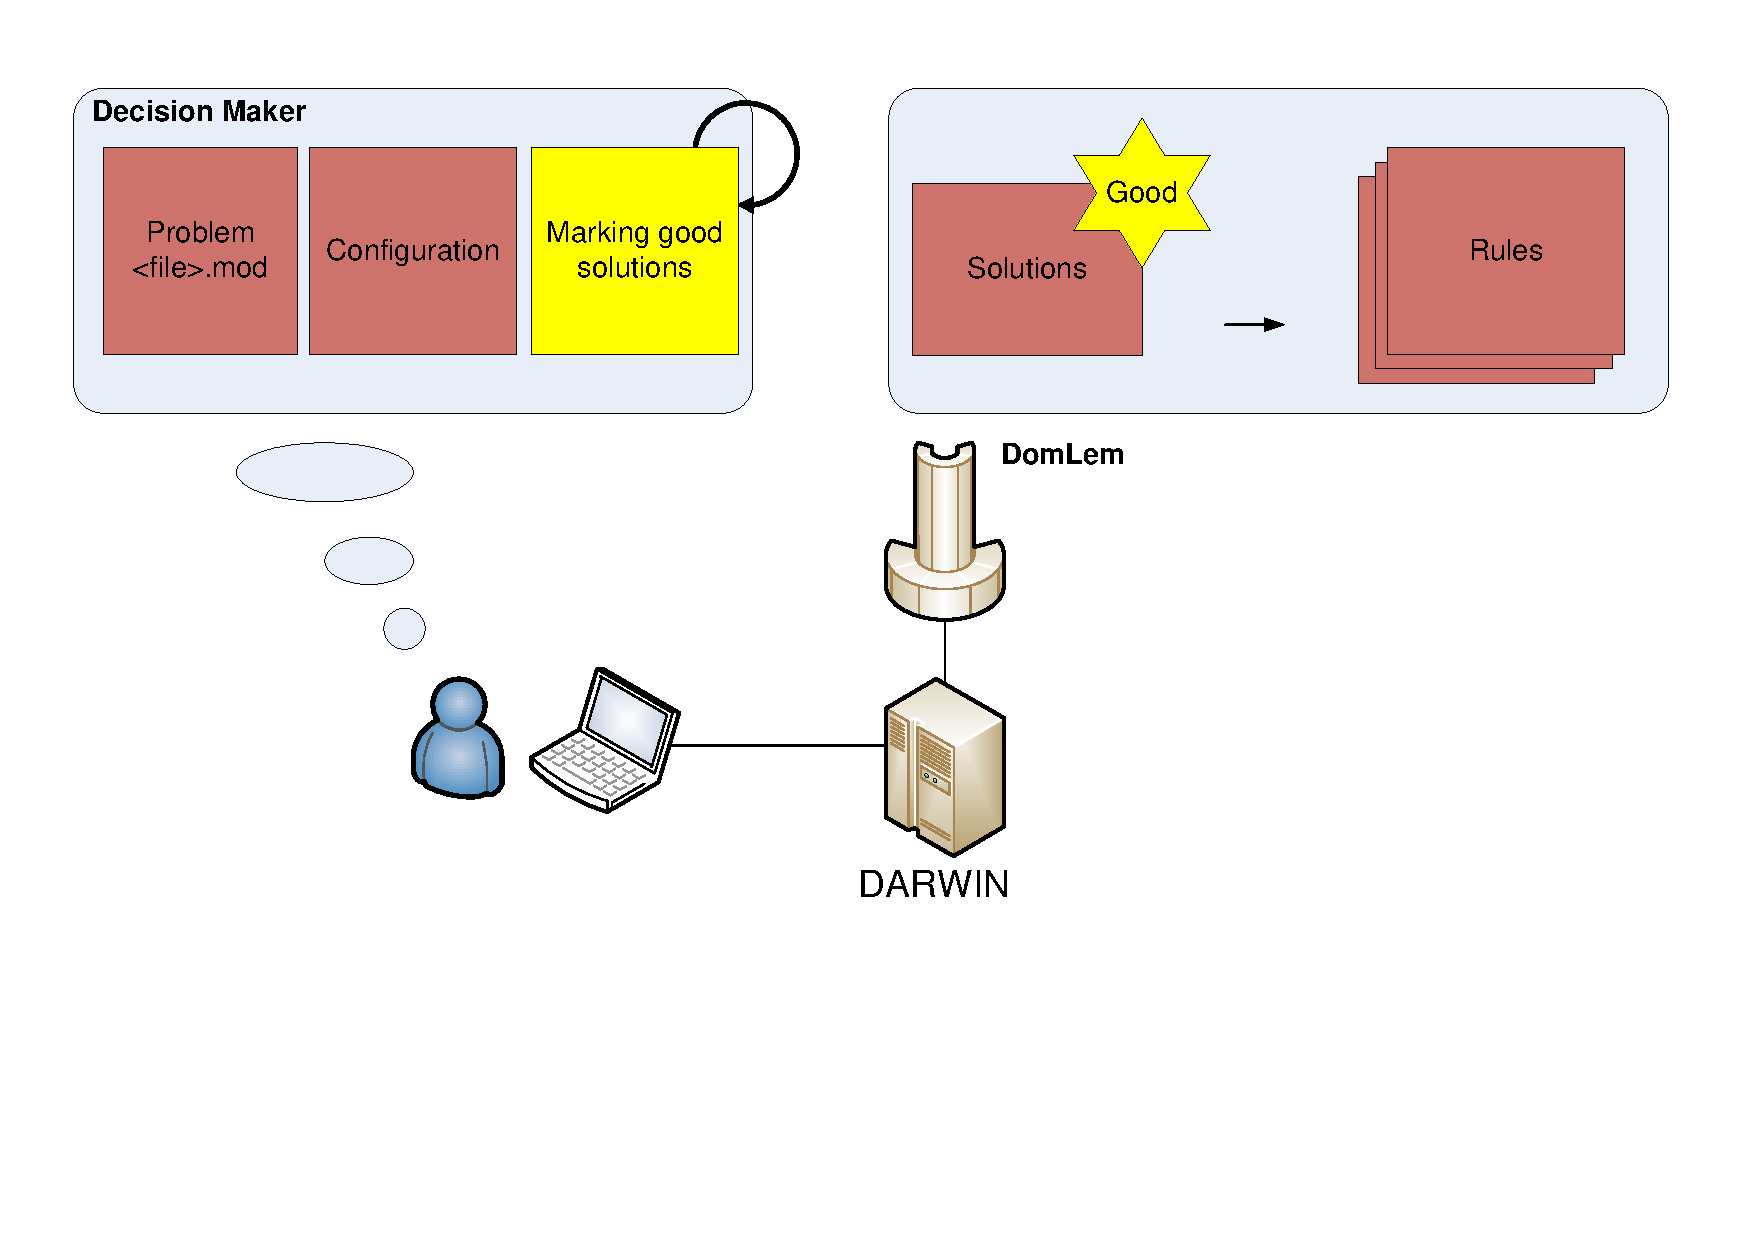
\includegraphics[scale=0.5]{img/environ}
  \caption{DARWIN's environment}
  \label{environ}
\end{figure}

The DM has to provide a problem he wants to solve. It can be done in a model
file. If one wants to change the default parameters' values a~configuration
file with the values is also required. Moreover, during the algorithm run,
presence of the decision maker is required, in order to select ``good''
solutions from the provided ones. Consult the user manual ([inref]) for more
details on the file formats. The parameters are described later in this
section.

Decision rules store the decision maker preferences, therefore they are
a~symbolic representation of trade-offs he or she is willing to make, as well
as the importance of an each criterion. They are ensuring a~robustness of the
resulting solutions because of an underlying DRSA framework. Te rules are
a~very important part of the method. Thus, a~way --- an algorithm --- to
generate them is need. In the method description a~phase of obtaining the
rules is treated as a~black-box. It is assumed that a~component able to
generate rules from the DM's selection exists. Details are omitted --- it is
up to analyst (or to a~developer of an implementation) to use a~software
component he or she will find feasible.

An implementation of the DRSA framework, being able to induce decision rules
from a~given set of examples is a complex task. Both in terms of possible
technical challenges as well as a~conceptual and a~scientific work that needs
to be carried. Such a software application deserves a paper of its
own. Therefore, the author decided to use an existing implementation in order
to focus on the DARWIN method. Java Rough Set (jRS) --- a~project of the
Laboratory of Intelligent Decision Support Systems at Poznań University of
Technology, that aims at providing DRSA framwork implementation in Java ---
was chosen. It contains the DomLem algorithm able to generate a~minimal set of
decision rules from the examples given as its input.

jRS is written in Java programming language ([ref]) and runs on top of the
Java Virtual Machine (JVM, [ref]). The JVM is a~portable platform capable of
running the Java bytecode. However, the technical details of the Java platform
are out-of-scope of this article. Having a~Java component (jRS in this case)
effectively put a~constraint on the DARWIN implementation --- it is required
that the implementation is also delivered as a JVM application.

\subsection{The prototype}

As his first task, the author choose to implement a prototype of the
program. The goal was to check the behavior of the method --- if it works,
coverages to the preferred region, is able to generate reasonable solution and
to withstand the uncertainty in the decision makers preferences. If the
overview given in~[ref] is accurate enough to develop a~working software. More
important however, was to find out potential problems and to gain a deep
knowledge of the method.

The prototype was developed in Java. Java is a very popular language and de
facto an industry standard in many fields, especially in enterprise
applications. The application itself is able to solve a subset of the MMO
problems. It supports uncertainty and it mocks the decision maker. It is a
working implementation of the method. The goal was achieved --- to develop
a~working piece of software showing that DARWIN is able to solve
multi-objective optimization problems. 

Unfortunately, the prototype has not been fully featured. It has contained
only a mocked DM and laked any user interface at all. The problem to solve and
the DARWIN parameters are hard-coded for the prototype. Nevertheless, the code
was being developed in extensible way and contained a suite of
unit-tests. However, it is a~common practice in the software engineering to
discard the prototype and start developing the final application from scratch.
This was the case with DARWIN --- the author's knowledge of the method changed
during the prototyping and starting from the beginning has been considered
a~better option.

\subsection{The final implementation}
The Java language is stable, well tested and features numerous libraries
dedicated to almost any possible application; unfortunately, it is also very
verbose and lacks support for many of recent trends in the software
engineering. It is a great tool for large teams, which is usually the case in
enterprise application development. However, what is a good solution for
a~team is not essentially the best possible tool for a~single developer
working on a~project.

The author decided to develop the implementation in Scala ([ref]). Scala is a
multi-paradigm programming language combining object-oriented features with
functional programming. The former dominates on the contemporary
software-development market and allows to program and model problem domain's
objects as well as relations between them, however the latter is very useful
in writing concise code dealing with mathematical computations. This is a~very
useful trait in a~scientific project like DARWIN.

Scala runs on JVM, therefore it is compatible with existing Java
libraries. The Scala compiler produces a java bytecode from a Scala source
code. The bytecode is nearly identical as the one generated from a Java
source. The only difference is that Scala programmes require a presence of an
additional run-time library --- \textit{scala-library.jar}. The launguage was
designed by Martin Odersky and started as a project in École Polytechnique
Fédérale de Lausanne (EPFL, [ref]). Because of the functional elements and
different syntax Scala programs are usually sorter and easier to read that
their Java counterparts, especially when dealing with mathematical operations.

The code is divided into packages. Their structure is shown in
fig.~\ref{packages}.

\begin{figure}
  \centering 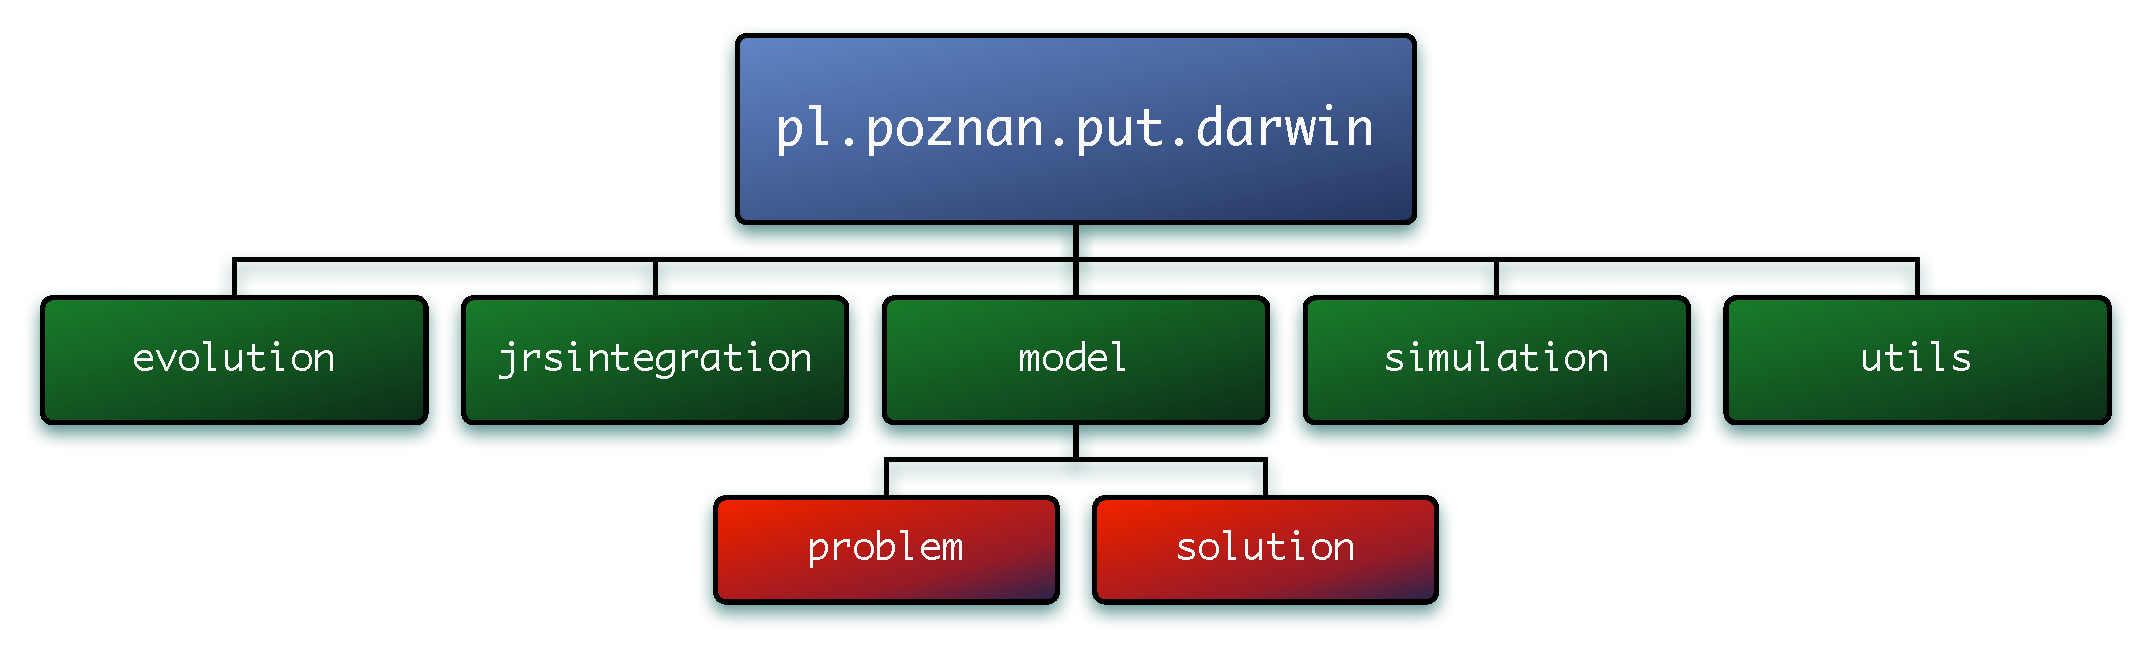
\includegraphics[scale=0.9]{img/packages}
  \caption{The package structure of DARWIN}
  \label{packages}
\end{figure}


\subsection{Configurable parameters}


\section{Experiment framework}
